\chapter{Evaluation}
\label{cha:eval}
One of the main aims of my project is the evaluation of results...

\section{Transmission delay}
\label{sec:eval_comm_rel}

According to my experiments, sending SDP packets immediately between two cores results on a very large packet drop ration. Without explicit delay between the transmission of packets, the number of successful deliveries is only about 10\% of those sent for a large number of packets. This effect is strongly reduced by the addition of a small delay of 5-10$\mu$s, which guarantees over 99\% successful deliveries, as can be seen on table \ref{table:sdp_deliveries}. The table also shows that having long delays, greater than 10$\mu$s is mostly redundant, as they do not decrease packet loss significantly, but tragically reduce throughput.

Upon experimenting, I found that sending a large amount of consecutive, immediate packets (at least 1,000,000) has a chance of consequently crashing the destination core or causing it to reach the erraneous watchdog state (WDOG), meaning it cannot respond to commands.

\begin{table}
\begin{tabular}{ r | c | c | c | c | c }
Packets sent & no delay & 2µs delay & 5µs delay & 10µs delay & 100µs delay \\
50,000 & 9.56\% & 57.73\% & 95.95\% & 98.36\% & 99.85\% \\
100,000 & 12.15\% & 54.97\% & 97.99\% & 99.13\% & 99.92\% \\
200,000 & 13.07\% & 50.55\% & 99.01\% & 99.33\% & 99.96\% \\
500,000 & 12.97\% & 50.08\% & 99.49\% & 99.80\% & 99.99\% \\
1,000,000 & 13.05\% & 45.06\% & 98.84\% & 99.88\% & 99.99\% \\
\end{tabular}
\caption{Successful SDP deliveries with delay between each packet}
\label{table:sdp_deliveries}
\end{table}

Note that the experiment, made on SpiNN-3, involved sending a single point-to-point packet multiple times to the same destination, containing only the 8 byte SDP header. The destination did not store or read the packet contents, only incrementing a counter upon packet receival. This was used to show the maximum possible transmission rate allowed by the SDP protocol under the hardware communication fabric. Code snippets and more information can be found on the appendix under section \ref{sec:appendix_comm_rel}.

Ideally these packets would send useful information, to be read upon arrival, which would keep the destination busy. From my experience and input from the team, the best way to achieve this is by immediately storing the SDP packet contents into a buffer when it is received and then handling it at a different point in time (listing \ref{lst:sdp_packet_callback}). The reason for this is that if another packet arrives as we are processing the current packet with same or higher priority, the incomming packet will drop.

Ideally high priority should be assigned to storing incomming packets into a buffer and the actual processing should have lower priority, as it can be handled at a later point in time. It is important to note that this can cause starvation and buffer overflow if there are too many immediate packets being received. For instance, if our SDP packet is of size 12-byte (8-byte header + 32-bit data) and stored into a buffer in DTCM upon receival, we would only ever be able to hold up to about 5,000 messages at once (64-Kbytes DTCM size / 12-byte packet size). Realistically a large part of DTCM contains the stack, local and global variables, so that number will be drastically reduced. In my application, SpiDB, insert and retrieve database queries have a size of 256-bytes, which means a limit of 250 entries in the buffer if DTCM were empty.

This evaluation is important because it allows finding the optimal transmission delay for an application. A developer on SpiNNaker using the point-to-point protocol needs to find the balance between transmission rate and reliability, which are inversely proportional. This balance is application dependent.

\lstinputlisting[language=C, caption=Storing incomming packets into a queue, label={lst:sdp_packet_callback}]{code/sdp_packet_callback.c}

On SpiDB, I experimented with different time delays when transmitting packets from host over ethernet to a core on SpiNNaker, in order to find the best evaluation. The speed of one operation is calculated as the time of successful reply minus the time that operation was sent from host, thus being a round-trip-time plus internal processing time. The performance is calculated as the amount of operations successfully executed in one second.

As can be seen on figure \ref{fig:transmission-delay}, large packet transmission delays of 50-100$\mu$s cause only a bottleneck, as they do not reduce packet drops, while being a high cost on performance. Naturally the more packets we can send in one second influences the speed of replies, thus improving performance. This hits a maxima at 40$\mu$s, with almost 10,000 op/sec, in which transmission is at a high rate with no loss of reliability. Transmission delays between 40-10$\mu$s result on a decrease of performance, because although packets are sent more frequently, a lot of them are dropped (up to about 35\%), being also extremely unreliable. We reach the worst case at 10-5$\mu$s delay, when the destination core cannot cope with the speed on incomming packets, simply crashing and ceasing to respond. This SpiDB experiment was performed with 100,000 \textit{put} operations with keys and values of size 4-bytes each. More information on the data gathered can be found on the appendix under section \ref{sec:appendix_comm_rel}.

\begin{figure}
\begin{center}
	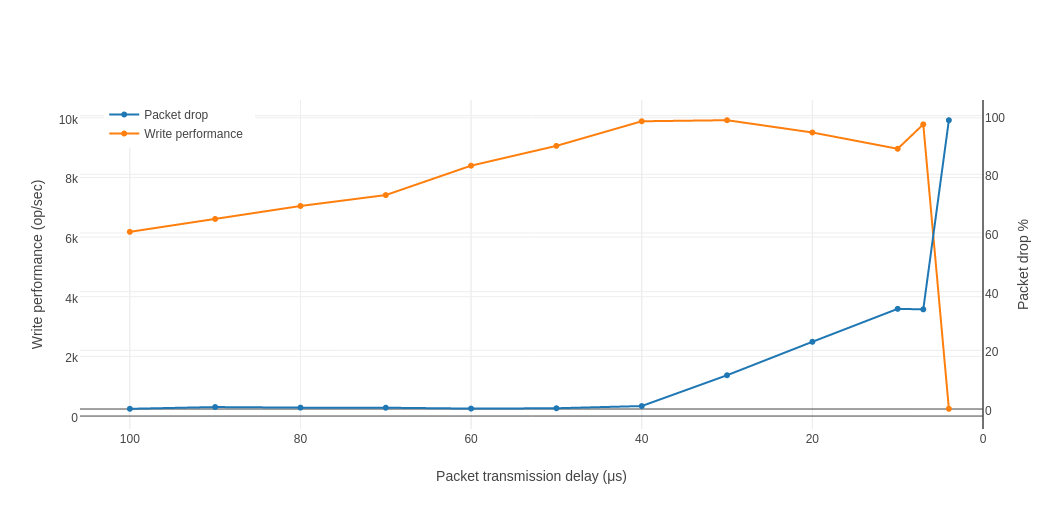
\includegraphics[width=1.4\textwidth, natwidth=1063, natheight=509]{images/transmission_delay.png}
\end{center}
\caption{Transmission delay plot}
\label{fig:transmission-delay}
\end{figure}

put operations

acknowledgements

 improve

THIS TAKES 1microsecond using the watchdog timer.

callback priorities etc.

cannot possibly do more than that...????
ARM968 at only 180MHz (I think)

response times. why are they so high sometimes?!?!
-first explain how we gather the time (operating system could be interrupting, sark, etc.)


In the assumption that the programmer needs to store XX into a buffer XXX
at least 32 bits of data, that means the packet size of 12 bytes.


The SpiNNaker communication fabric is known for being unreliable, which reflects the way the human brain acts, in a way that neuron spikes are not reliable... (why???)

single source, multiple destinations is also bad!

why does this happen?

single source, multiple destinations


WHY


always lose 77...

maybe more reliability with a layer on top of UDP, which would be more expensive/slow



aim: balance of memory and processing power on the chip, etc.


This would ideally allow a linear speedup of data retrival in comparison with a sequential system.


\section{Performance benchmark}

Comparison with two of the most popular RAM-based Key-value pair databases: \textbf{memcached} and \textbf{Redis}.
Run on an ASUS X555L quadcore Intel(R) Core(TM) i5-5200U CPU @ 2.20GHz, 8gb DDR3 RAM @ 1600 MHz.

Write speed with different data sizes, etc.

256 is the limit data size of sdp messages...

As can be seen in figure XXX, the SpiNNaker Database (SpiDB) on the 4 chip board performs quite poorly against the two, running at around 7k put operations per second, compared to ... (thus slow by a factor of about 8) 

complexity

hash vs naive

HOW ABOUT ALL SEQUENTIAL (dots) VS ALL PARALLEL????

\section{Limitations}

\section{Predictions}

\section{Future work}
future work...
cache (on DTCM)
aggregation
CGI server
self balancing when IDLE (ie. move data to cores with less data, if a table is about to get full, move data around it's SDRAM) --- user typing = a long time
million core machine
improve parser
allow longer queries in (more than 256 bytes)
additional operations eg. delete, update, etc,...
more reliability
ACID properties